% Source: graduate-coursework/Prior_Semesters/Fa25/EMCH721/solution_hw3.tex

\documentclass[border=4pt]{standalone}
\usepackage{amsmath}
\usepackage{amssymb}
\usepackage{graphicx}
\usepackage{pgfplots}
\usepackage{tikz}
\usepackage{xcolor}
\pgfplotsset{compat=1.18}
\usetikzlibrary{shapes.geometric, arrows.meta, positioning, decorations.pathmorphing, patterns, calc}

\definecolor{USC_Garnet}{HTML}{73000A}
\definecolor{USC_Sandstorm}{HTML}{FFF2E3}
\definecolor{USC_Black90}{HTML}{565656}
\definecolor{USC_Black10}{HTML}{ECECEC}
\definecolor{USC_Honeycomb}{HTML}{65780B}

\newcommand{\solutionframework}{%
\subsection*{Solution Outline}
\begin{stepbox}
\textbf{Planned Steps}\\[0.5em]
Outline your step-by-step approach here.
\end{stepbox}
\subsection*{MATLAB Implementation}
\begin{codebox}
Add MATLAB code or pseudocode here.
\end{codebox}
\subsection*{Results Summary}
\begin{resultsbox}
Summarize key intermediate and final results here.
\end{resultsbox}
}

\begin{document}
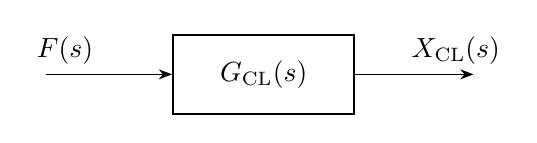
\begin{tikzpicture}[auto,>=Stealth,node distance=2.2cm,block/.style={draw,thick,rectangle,minimum height=1cm,minimum width=2.3cm}]
  \node[coordinate] (r) {};
  \node[block,right=1.6cm of r] (gcl) {$G_{\text{CL}}(s)$};
  \node[coordinate,right=1.5cm of gcl] (x) {};
  \draw[->] (r) -- node[pos=0.15,above] {$F(s)$} (gcl);
  \draw[->] (gcl) -- node[pos=0.85,above] {$X_{\text{CL}}(s)$} (x);
\end{tikzpicture}
\end{document}
